\documentclass[conference]{IEEEtran}

% IEEEtran v1.8b (2015) — clase oficial para conferencias IEEE.
% Documentaci\'on: https://www.michaelshell.org/tex/ieeetran/
% Nota: el paquete geometry sobreescribe los m\'argenes de IEEEtran.

\IEEEoverridecommandlockouts
% Permite usar \thanks en modo conference (bloqueado por defecto en IEEEtran).

\usepackage{times}
\usepackage[T1]{fontenc}
\usepackage[utf8]{inputenc}
\usepackage[spanish,es-tabla,es-noshorthands]{babel}
% es-noshorthands: evita que babel-spanish active ~ como car\'acter especial,
% lo cual rompe comandos de IEEEtran y el uso de \~n en nombres.

\usepackage{graphicx}
\usepackage{amsmath}
\usepackage{amssymb}
\usepackage{cite}
\usepackage{tikz}
\usetikzlibrary{positioning, arrows.meta, shapes, fit, backgrounds, calc}

% hyperref DEBE cargarse al final para evitar conflictos con cite, amsmath, etc.
\usepackage[bookmarks=false]{hyperref}
\hypersetup{
  colorlinks=false,
  pdfborder={0 0 0},
  linkcolor=black,
  citecolor=black,
  urlcolor=black
}
\urlstyle{same}

% Geometry: sobreescribe m\'argenes IEEEtran
\usepackage[letterpaper, top=19mm, bottom=25.4mm, left=17.3mm, right=17.3mm, columnsep=4.22mm]{geometry}

\begin{document}

\title{An\'alisis de la Resiliencia Operativa en Pipelines de CI/CD: Automatizaci\'on de Mecanismos de Rollback ante Despliegues Degradados mediante Infraestructura como C\'odigo}

\author{\IEEEauthorblockN{Jhon Cruz Tairo}
\and
\IEEEauthorblockN{Daren Herrera Romo}
}

\maketitle

\pagestyle{empty}
\thispagestyle{empty}
% Sin n\'umeros de p\'agina, sin encabezados ni pies.

\begin{abstract}
La integraci\'on y entrega continuas (CI/CD) constituyen un pilar del paradigma DevOps y aceleran el ritmo de despliegue, pero incrementan la probabilidad de que versiones defectuosas alcancen producci\'on, lo cual exige mecanismos de reversi\'on autom\'atica que minimicen el tiempo de recuperaci\'on. En este trabajo se documenta un experimento controlado que compara dos estrategias de detecci\'on de fallos ---umbral fijo de fallos consecutivos y ventana deslizante de observaci\'on--- en un pipeline CI/CD con cuatro tipos de fallo inyectados, contrastando los resultados contra una intervenci\'on manual de referencia. Se ejecutaron 110 corridas independientes sobre un servicio web desplegado con Docker y gestionado con infraestructura como c\'odigo mediante Terraform, en un entorno aislado y reproducible. La estrategia de ventana deslizante registr\'o un MTTR promedio entre 25.6~s y 26.9~s, frente a valores entre 32.9~s y 35.0~s para el umbral fijo y entre 38.8~s y 40.3~s para la intervenci\'on manual. La tasa de detecci\'on fue del 100~\% en todas las combinaciones, sin falsos positivos ni falsos negativos. La reducci\'on del MTTR respecto a la intervenci\'on manual alcanz\'o un promedio del 33.0~\%. Estos resultados proporcionan evidencia emp\'irica para la selecci\'on de pol\'iticas de monitoreo en pipelines de despliegue automatizado.
\end{abstract}

\renewcommand{\IEEEkeywordsname}{Index Terms}
\begin{IEEEkeywords}
CI/CD, reversi\'on autom\'atica, tiempo medio de recuperaci\'on, detecci\'on de fallos, infraestructura como c\'odigo, resiliencia operativa.
\end{IEEEkeywords}

\section{Introducci\'on}

La integraci\'on y entrega continuas han consolidado la pr\'actica de desplegar software con alta frecuencia y en ciclos reducidos, constituyendo uno de los pilares del paradigma DevOps~\cite{humble2010continuous, kim2016devops}. En este modelo, cada cambio de c\'odigo atraviesa un pipeline automatizado de compilaci\'on, verificaci\'on e implementaci\'on, con el objetivo de reducir el intervalo entre el desarrollo de una funcionalidad y su disponibilidad en producci\'on. Sin embargo, la aceleraci\'on del ritmo de despliegue incrementa simult\'aneamente la probabilidad de que una versi\'on defectuosa alcance el entorno operativo, especialmente cuando las pruebas automatizadas no logran detectar todos los modos de fallo~\cite{yuan2014simple}.

La literatura de ingenier\'ia de sistemas distingue entre la prevenci\'on de fallos durante la etapa de desarrollo y la capacidad de recuperaci\'on ante fallos que ya se han manifestado en producci\'on~\cite{basiri2016chaos}. Mientras que la primera se aborda con pr\'acticas de prueba exhaustiva, la segunda ---conocida como resiliencia operativa--- depende de mecanismos de supervisi\'on continua y de reversi\'on autom\'atica (\textit{rollback}) hacia un estado previamente estable. 

El vac\'io que motiva el presente experimento radica en la ausencia de evidencia comparativa: si bien se reconoce que la reversi\'on autom\'atica reduce el tiempo de recuperaci\'on con respecto a la intervenci\'on manual~\cite{challa2024selfhealing}, permanece sin resolver la pregunta de qu\'e estrategia de detecci\'on ---umbral fijo de fallos consecutivos frente a ventana deslizante de observaci\'on--- minimiza el tiempo medio de recuperaci\'on (MTTR) y con qu\'e costo en t\'erminos de falsos positivos.

En este contexto, el objetivo del presente trabajo es documentar un dise\~no experimental controlado que mida la efectividad de la reversi\'on autom\'atica de despliegues degradados en un pipeline CI/CD, comparando dos estrategias de detecci\'on de fallos y contrastando el resultado contra una intervenci\'on manual de referencia. El aporte de este art\'iculo no reside en la presentaci\'on de una herramienta nueva ni de un algoritmo de reversi\'on original, sino en la construcci\'on de una matriz comparativa de tipos de fallo frente a estrategias de detecci\'on, sustentada en repeticiones estad\'isticas y variables de control expl\'icitas. El resto del documento se organiza de la siguiente manera: la secci\'on II.A presenta el marco te\'orico que sustenta los conceptos de resiliencia, supervisi\'on con umbrales y anatom\'ia de la reversi\'on; la secci\'on II.B describe el dise\~no experimental, incluyendo las variables independientes, dependientes y de control; la secci\'on II.C expone los resultados cuantitativos obtenidos; la secci\'on II.D interpreta dichos resultados, los contrasta con el trabajo relacionado y declara las amenazas a la validez del experimento; finalmente, la secci\'on III formula las conclusiones del estudio.

\section{Desarrollo de Contenidos}

\subsection{Marco Te\'orico}

La pr\'actica de integraci\'on y entrega continuas se ha documentado como uno de los pilares operativos del paradigma DevOps, en el que un pipeline automatizado ejecuta secuencialmente las etapas de compilaci\'on, prueba e implementaci\'on, proporcionando retroalimentaci\'on inmediata sobre la viabilidad de cada cambio de c\'odigo~\cite{humble2010continuous}. Leite et al.~\cite{leite2017analysis}, en su revisi\'on sistem\'atica de la literatura de DevOps, identifican la automatizaci\'on del flujo de despliegue como uno de los conceptos centrales recurrentes en las pr\'acticas documentadas de integraci\'on y entrega continuas. Subramanya et al.~\cite{subramanya2022devops} subrayan que el monitoreo continuo constituye uno de los principios fundamentales de DevOps, ya que posibilita la observaci\'on del comportamiento del sistema en el entorno operativo y la identificaci\'on de desviaciones respecto a la l\'inea base de comportamiento normal. Esta visi\'on implica que el pipeline no concluye en el momento del despliegue, sino que se extiende hacia una fase de supervisi\'on que valida la correcta operaci\'on de la versi\'on reci\'en implementada.

Sin embargo, la aceleraci\'on del ritmo de despliegue conlleva un incremento simult\'aneo de la probabilidad de que versiones defectuosas alcancen producci\'on. Yuan et al.~\cite{yuan2014simple}, tras analizar fallos cr\'iticos en sistemas distribuidos de procesamiento intensivo de datos, concluyen que la mayor\'ia de dichos fallos podr\'ian haberse evitado con pruebas simples, lo cual revela un l\'imite inherente a las estrategias de prevenci\'on exclusivas: las pruebas automatizadas, por exhaustivas que sean, no detectan todos los modos de fallo posibles. Esta constataci\'on orienta la atenci\'on hacia la segunda l\'inea de defensa: la capacidad del sistema de recuperarse ante fallos que ya se han manifestado, en lugar de depender \'unicamente de evitar que ocurran.

La disciplina del chaos engineering formaliza esta transici\'on desde la prevenci\'on hacia la tolerancia a fallos. Basiri et al.~\cite{basiri2016chaos} definen el chaos engineering como la pr\'actica de experimentar sobre un sistema en producci\'on para generar confianza en su capacidad de soportar condiciones turbulentas, distingui\'endose de las pruebas tradicionales en que no busca validar comportamientos esperados, sino descubrir propiedades emergentes del sistema ante perturbaciones no anticipadas. Monge y Mat\'ok~\cite{monge2020developing} extienden esta perspectiva al contexto del desarrollo de software, proponiendo herramientas de inyecci\'on de fallos que permiten medir la resiliencia mediante la observaci\'on del comportamiento del sistema ante condiciones de estr\'es controladas. En ambos casos, la premisa subyacente es que la resiliencia no se demuestra mediante la ausencia de fallos, sino mediante la capacidad de recuperaci\'on ante ellos.

Los principios de resiliencia se trasladan a la operaci\'on automatizada de pipelines mediante el concepto de auto-reparaci\'on (\textit{heal-on-failure}). Challa y Konatham~\cite{challa2024selfhealing} proponen una arquitectura de pipeline auto-reparable que integra una capa de detecci\'on de anomal\'ias en tiempo real con un controlador de decisi\'on que activa la reversi\'on autom\'atica hacia el \'ultimo estado estable conocido. Su trabajo reporta mejoras superiores al 50\% en el tiempo medio de recuperaci\'on respecto a la intervenci\'on manual, aunque no desglosa los resultados por tipo de fallo ni compara pol\'iticas de detecci\'on alternativas. Avuthu~\cite{avuthu2021change} complementa esta visi\'on al analizar estrategias de reversi\'on basadas en infraestructura como c\'odigo, distinguiendo entre reversi\'on manual, reversi\'on automatizada, despliegue blue-green y despliegue canario, cada una con diferentes compromisos entre complejidad de implementaci\'on y tiempo de recuperaci\'on.

La efectividad de cualquier mecanismo de reversi\'on depende de la pol\'itica de detecci\'on que decide cu\'ando declarar un estado degradado. Hrusto et al.~\cite{hrusto2022optimization} estudian la optimizaci\'on de la detecci\'on de anomal\'ias en sistemas de microservicios mediante retroalimentaci\'on continua desde los equipos de desarrollo, se\~nalando que la elecci\'on del umbral de decisi\'on constituye un compromiso entre sensibilidad (capacidad de detectar fallos reales) y especificidad (capacidad de evitar alarmas falsas). En este contexto, el umbral fijo de fallos consecutivos representa la pol\'itica m\'as simple: se establece un n\'umero predeterminado de verificaciones fallidas consecutivas que, al alcanzarse, activa la reversi\'on. Su simplicidad facilita su implementaci\'on, aunque su rigidez puede generar reversiones innecesarias ante fluctuaciones transitorias.

Como alternativa al umbral fijo, la ventana deslizante de observaci\'on incorpora memoria temporal a la decisi\'on. En lugar de exigir fallos consecutivos, esta pol\'tica eval\'ua una proporci\'on de fallos dentro de un intervalo de observaci\'on deslizante, lo cual permite tolerar fallos aislados (por ejemplo, un timeout puntual por congesti\'on de red) sin activar una reversi\'on, detectando al mismo tiempo una tendencia consistente al fallo. La distinci\'on entre ambas pol\'ticas no reside en el mecanismo de instrumentaci\'on, que puede ser id\'entico, sino en la l\'ogica de decisi\'on que interpreta las se\~nales de supervisi\'on. Hrusto et al.~\cite{hrusto2022optimization} se\~nalan que las pol\'ticas que incorporan contexto temporal absorben mejor las fluctuaciones breves sin comprometer la capacidad de detectar fallos persistentes, aunque su an\'alisis se centra en m\'etodos de aprendizaje profundo para la detecci\'on de anomal\'ias, no en pol\'ticas de umbral simples como las que se comparan en este trabajo.

El tiempo medio de recuperaci\'on (MTTR) constituye uno de los indicadores clave del rendimiento de entrega de software en la literatura de DevOps. Kim et al.~\cite{kim2016devops} reportan, a partir de datos de m\'as de veinticinco mil profesionales de tecnolog\'ia, que las organizaciones de alto rendimiento logran tiempos de restauraci\'on 168 veces menores que sus pares de bajo rendimiento, vinculando esta capacidad directamente con la adopci\'on de pr\'acticas DevOps que incluyen la reversi\'on automatizada. Challa y Konatham~\cite{challa2024selfhealing} emplean el MTTR como m\'etrica principal para evaluar la efectividad de su arquitectura auto-reparable, mientras que Avuthu~\cite{avuthu2021change} lo utiliza para comparar el desempe\~no de las diferentes estrategias de reversi\'on. La duraci\'on total del ciclo de detecci\'on, decisi\'on y ejecuci\'on de la reversi\'on constituye, en todos estos trabajos, la medida est\'andar de efectividad operativa.

Si bien la literatura citada reconoce la importancia de la reversi\'on autom\'atica, propone arquitecturas para su implementaci\'on y utiliza el MTTR como m\'etrica de evaluaci\'on, persiste una carencia de estudios comparativos que midan el desempe\~no de diferentes pol\'ticas de detecci\'on bajo un mismo dise\~no experimental, con repeticiones estad\'isticas y un grupo de referencia manual. Challa y Konatham~\cite{challa2024selfhealing} reportan mejoras agregadas sin desglose por categor\'ia de fallo; Avuthu~\cite{avuthu2021change} describe estrategias de reversi\'on pero no proporciona datos experimentales de comparaci\'on; y Hrusto et al.~\cite{hrusto2022optimization} se centran en m\'etodos de aprendizaje profundo para la detecci\'on, no en pol\'ticas de umbral de decisio\'n simples. El presente trabajo se sit\'ua en este vac\'io metodol\'ogico, adoptando un enfoque que no introduce nuevas t\'ecnicas de detecci\'on ni nuevos mecanismos de reversi\'on, sino que compara cuantitativamente dos pol\'ticas existentes de decisi\'on de degradaci\'on bajo condiciones controladas, con el objetivo de aportar evidencia emp\'irica para la selecci\'on de pol\'ticas de monitoreo en pipelines de despliegue.

\subsection{Metodolog\'ia / Dise\~no Experimental}

El experimento se organiz\'o como un dise\~no factorial completo en el que se combinaron cuatro tipos de fallo inyectado con dos estrategias de detecci\'on de degradaci\'on, adem\'as de un grupo de referencia con intervenci\'on manual y un conjunto de corridas de control. En total se ejecutaron 110 corridas independientes: 80 autom\'aticas (4 fallos por 2 estrategias por 10 repeticiones), 20 de baseline manual (4 fallos por 5 repeticiones) y 10 de control sin fallo (2 estrategias por 5 repeticiones). En las corridas de control se despleg\'o la versi\'on estable sin ninguna modificaci\'on, con el fin de verificar que ninguna de las dos estrategias activara una reversi\'on en ausencia de fallo. Cada corrida fue independiente de la anterior; el contenedor se destruy\'o y se volvi\'o a desplegar desde cero entre una y otra, eliminando cualquier efecto de estado residual.

El entorno de ejecuci\'on se implement\'o sobre un sistema operativo invitado en una m\'aquina virtual ligera. Los despliegues se gestionaron mediante un motor de contenedores, y la configuraci\'on de cada versi\'on se declar\'o a trav\'es de una herramienta de infraestructura como c\'odigo. El servicio bajo prueba expuso un endpoint de verificación de salud que constituy\'o la \'unica fuente de informaci\'on para las estrategias de detecci\'on. Todas las corridas compartieron la misma configuraci\'on de red, el mismo intervalo de consulta de salud, fijado en 5 segundos, y el mismo tiempo m\'aximo de espera por verificaci\'on, fijado en 2 segundos.

Se definieron cuatro categor\'ias de fallo, cada una materializada mediante una modificaci\'on deliberada del artefacto de construcci\'on o de la configuraci\'on de despliegue. El primero consisti\'o en una instrucci\'on inv\'alida en el archivo de construcci\'on de la imagen, lo cual imped\'ia la creaci\'on del contenedor. El segundo expuso el servicio en un puerto distinto al que el mecanismo de verificaci\'on de salud consultaba; el contenedor se ejecutaba pero resultaba inalcanzable. El tercero introdujo una latencia de respuesta superior al tiempo de espera configurado, simulando una condici\'on de agotamiento de recursos. El cuarto, finalmente, omiti\'o una variable de entorno requerida por el servicio, provocando que este respondiera con un c\'odigo de error interno.

\begin{figure}[t]
\centering
\begin{tikzpicture}[
  box/.style={draw, rectangle, thick, minimum width=1.6cm, minimum height=0.55cm, align=center, font=\footnotesize, inner sep=2pt},
  arrow/.style={-{Stealth[scale=0.7]}, thick}
]
  \node[box, minimum width=1.2cm] (git)   at (0,    0)   {Git};
  \node[box]                      (pipe)  at (0,   -1.1)  {Pipeline};
  \node[box]                      (est)   at (-1.15,-2.0) {Estable};
  \node[box]                      (fall)  at (1.15,-2.0)  {Con fallo};
  \node[box]                      (serv)  at (0,   -3.2)  {Servicio};
  \node[box]                      (mon)   at (1.9, -3.2)  {Monitor};
  \node[box]                      (dec)   at (3.8, -3.2)  {Decisi\'on};
  \node[box]                      (roll)  at (3.8, -4.1)  {Rollback};
  \node[box]                      (ver)   at (3.8, -5.0)  {Verificar};

  \draw[arrow] (git.south)   -- (pipe.north);
  \draw[arrow] (pipe.210)    -- (est.north);
  \draw[arrow] (pipe.330)    -- (fall.north);
  \draw[arrow] (est.south)   -- (serv.155);
  \draw[arrow] (fall.south)  -- (serv.25);
  \draw[arrow] (serv.east)   -- (mon.west);
  \draw[arrow] (mon.east)    -- (dec.west);
  \draw[arrow] (dec.south)   -- (roll.north);
  \draw[arrow] (roll.south)  -- (ver.north);
  \draw[arrow, dashed] (dec.west) .. controls +(left:0.9cm) and +(up:0.3cm) .. (mon.south)
    node[midway, above, font=\tiny, color=gray] {bucle};
\end{tikzpicture}
\caption{Arquitectura del pipeline experimental. El flujo bifurca entre versi\'on estable y versi\'on con fallo. El monitor consulta el estado de salud cada 5 segundos y el motor de decisi\'on aplica la estrategia de detecci\'on activa.}
\label{fig:arquitectura}
\end{figure}

Se compararon dos pol\'iticas de decisi\'on para determinar cu\'ando declarar el estado degradado. La primera, denominada de umbral fijo, activaba la reversi\'on tras tres verificaciones consecutivas fallidas, sin tolerancia a fallos aislados. La segunda, denominada de ventana deslizante, evaluaba una proporci\'on de fallos dentro de una ventana de seis verificaciones; si al menos tres de ellas resultaban negativas, se declaraba el estado degradado y se disparaba la reversi\'on. En ambos casos, la reversi\'on consisti\'o en reaplicar la configuraci\'on de la versi\'on estable mediante la herramienta de infraestructura como c\'odigo, restaurando el contenedor a su estado operativo anterior. Ambas estrategias operaron sobre el mismo endpoint y con el mismo intervalo de consulta, de modo que las diferencias observadas fueran atribuibles exclusivamente a la l\'ogica de decisi\'on y no a la instrumentaci\'on.

El estado degradado se defini\'o como la ausencia de una respuesta exitosa desde el endpoint de salud dentro del tiempo de espera establecido. Para la estrategia de umbral fijo, tres fallos consecutivos descartaban la posibilidad de una fluctuaci\'on transitoria. Para la ventana deslizante, tres fallos dentro de seis verificaciones permit\'ian tolerar hasta dos fallos aislados sin activar la reversi\'on, en l\'inea con los rangos recomendados en la literatura para entornos con perfiles de fallo transitorio. La Fig.~\ref{fig:estrategias} ilustra la diferencia de comportamiento entre ambas pol\'iticas ante una misma secuencia de verificaciones.

\begin{figure}[t]
\centering
\begin{tikzpicture}[
  font=\footnotesize,
  hc/.style={minimum width=0.55cm, minimum height=0.55cm, font=\footnotesize\bfseries},
  ok/.style={hc, circle, draw=green!50!black, fill=green!20},
  fail/.style={hc, circle, draw=red!70!black, fill=red!20},
  label/.style={font=\tiny, align=center}
]
  % Spacing factor reduced to fit column width (~8.5 cm)
  % Health check numbers
  \foreach \x/\num in {1/1,2/2,3/3,4/4,5/5,6/6,7/7,8/8} {
    \node[font=\tiny, gray] at (\x*0.7, 2.4) {HC\num};
  }
  
  % Health check results: ✓ ✗ ✗ ✓ ✗ ✗ ✗ ✓
  \node[ok]   at (0.7, 1.9)  {$\checkmark$};
  \node[fail] at (1.4, 1.9)  {$\times$};
  \node[fail] at (2.1, 1.9)  {$\times$};
  \node[ok]   at (2.8, 1.9)  {$\checkmark$};
  \node[fail] at (3.5, 1.9)  {$\times$};
  \node[fail] at (4.2, 1.9)  {$\times$};
  \node[fail] at (4.9, 1.9)  {$\times$};
  \node[ok]   at (5.6, 1.9)  {$\checkmark$};
  
  % E1 label
  \node[anchor=east] at (-0.1, 1.2) {\textbf{E1:}};
  
  % E1 consecutive failures
  \node[label] at (0.7, 1.2) {0};
  \node[label] at (1.4, 1.2) {1};
  \node[label] at (2.1, 1.2) {2};
  \node[label] at (2.8, 1.2) {0};
  \node[label] at (3.5, 1.2) {1};
  \node[label] at (4.2, 1.2) {2};
  \node[label, red!80!black] at (4.9, 1.2) {\textbf{3}};
  \node[label] at (5.6, 1.2) {0};
  
  % E1 trigger arrow
  \draw[red, thick, -{Stealth}] (4.9, 0.85) -- (4.9, 0.5) node[below, font=\tiny, red!80!black] {Dispara en HC7};
  
  % E2 label
  \node[anchor=east] at (-0.1, -0.1) {\textbf{E2:}};
  
  % E2 window showing failures in last 6
  \node[label] at (0.7, -0.1) {1};
  \node[label] at (1.4, -0.1) {1};
  \node[label] at (2.1, -0.1) {2};
  \node[label] at (2.8, -0.1) {2};
  \node[label] at (3.5, -0.1) {3};
  \node[label, blue!80!black] at (4.2, -0.1) {3};
  \node[label, blue!80!black] at (4.9, -0.1) {3};
  \node[label] at (5.6, -0.1) {2};
  
  % Window bracket for HC5
  \draw[blue, thick, -{Stealth}] (3.5, -0.45) -- (3.5, -0.8) node[below, font=\tiny, blue!80!black] {Dispara en HC5};
  
  % Window bracket visual
  \draw[blue, thin, dashed] (0.35, -0.35) rectangle (3.85, 0.1);
  \node[font=\tiny, blue!50!black] at (2.1, 0.25) {ventana HC1--HC5: 3};
  
  % Legend (left-aligned to avoid overflow)
  \node[font=\tiny, gray, anchor=west] at (0.0, -1.1) {HC = verificaci\'on de salud};
\end{tikzpicture}
\caption{Comparaci\'on del comportamiento de ambas estrategias ante la secuencia de verificaciones HC1 a HC8. E1 cuenta fallos consecutivos y dispara en HC7 al alcanzar tres. E2 eval\'ua una ventana deslizante de seis verificaciones y dispara en HC5 al detectar tres fallos dentro de la ventana.}
\label{fig:estrategias}
\end{figure}

El grupo de referencia con intervenci\'on manual se dise\~n\'o para cuantificar el tiempo de recuperaci\'on sin automatizaci\'on. En cada corrida se simul\'o la actuaci\'on de un operador humano mediante una pausa fija, calibrada antes del experimento, seguida de la restauraci\'on manual de la configuraci\'on estable. La duraci\'on de la pausa representaba el intervalo necesario para que un operador diagnosticara el fallo y ejecutara la reversi\'on en el mismo entorno. No se incluyeron corridas de control para el baseline manual, dado que la intervenci\'on humana no se activa en ausencia de fallo.

Se registraron cuatro m\'etricas para cada corrida. El tiempo medio de recuperaci\'on se calcul\'o como la diferencia entre el momento en que la estrategia de detecci\'on declaraba el estado degradado y el momento en que el endpoint de salud confirmaba la restauraci\'on exitosa (ver Fig.~\ref{fig:estrategias} para la l\'ogica de cada estrategia). La tasa de detecci\'on correcta se calcul\'o como la proporci\'on de corridas en las que el fallo inyectado fue efectivamente detectado por la estrategia activa. Los falsos negativos se registraron cuando el fallo no fue detectado y el sistema permaneci\'o en estado fallido. Los falsos positivos se midieron exclusivamente en las corridas de control, en las que no se hab\'ia inyectado fallo alguno.

\subsection{Resultados}

Se completaron las 110 corridas del dise\~no factorial seg\'un lo programado. Los 80 despliegues con fallo inyectado fueron detectados correctamente, sin registrar falsos negativos. Las 10 corridas de control no produjeron falsos positivos en ninguna de las dos estrategias. Todas las recuperaciones fueron exitosas, verificadas mediante la obtenci\'on del c\'odigo 200 en el endpoint de salud tras la reversi\'on.

\begin{table}[t]
\caption{MTTR Promedio y Desviaci\'on Est\'andar (s) por Tipo de Fallo y Estrategia}
\label{tab:mttr}
\centering\footnotesize
\resizebox{\columnwidth}{!}{%
\begin{tabular}{lccc}
\hline
\textbf{Tipo de fallo} & \textbf{Umbral fijo} & \textbf{Ventana deslizante} & \textbf{Manual} \\
\hline
Sintaxis (build)     & $32.9 \pm 2.3$ & $26.8 \pm 3.3$ & $38.8 \pm 0.3$ \\
Puerto cerrado       & $34.1 \pm 0.7$ & $26.7 \pm 0.9$ & $39.5 \pm 0.3$ \\
Timeout health check & $34.5 \pm 1.3$ & $26.9 \pm 0.8$ & $39.8 \pm 0.5$ \\
Dependencia faltante & $35.0 \pm 1.5$ & $25.6 \pm 0.7$ & $40.3 \pm 0.7$ \\
\hline
\end{tabular}
}
\end{table}

La Tabla~\ref{tab:mttr} presenta el MTTR promedio y su desviaci\'on est\'andar para cada combinaci\'on. En los cuatro tipos de fallo, la estrategia de ventana deslizante registr\'o valores de MTTR menores que los de la estrategia de umbral fijo: entre 25.6~s y 26.9~s para la ventana deslizante, frente a entre 32.9~s y 35.0~s para el umbral fijo. La diferencia entre ambas estrategias, a favor de la ventana deslizante, oscil\'o entre 5.4~s (sintaxis) y 9.4~s (dependencia faltante). El baseline manual present\'o valores entre 38.8~s y 40.3~s, superiores en todos los casos a los tiempos de ambas estrategias autom\'aticas.

\begin{figure}[t]
\centering
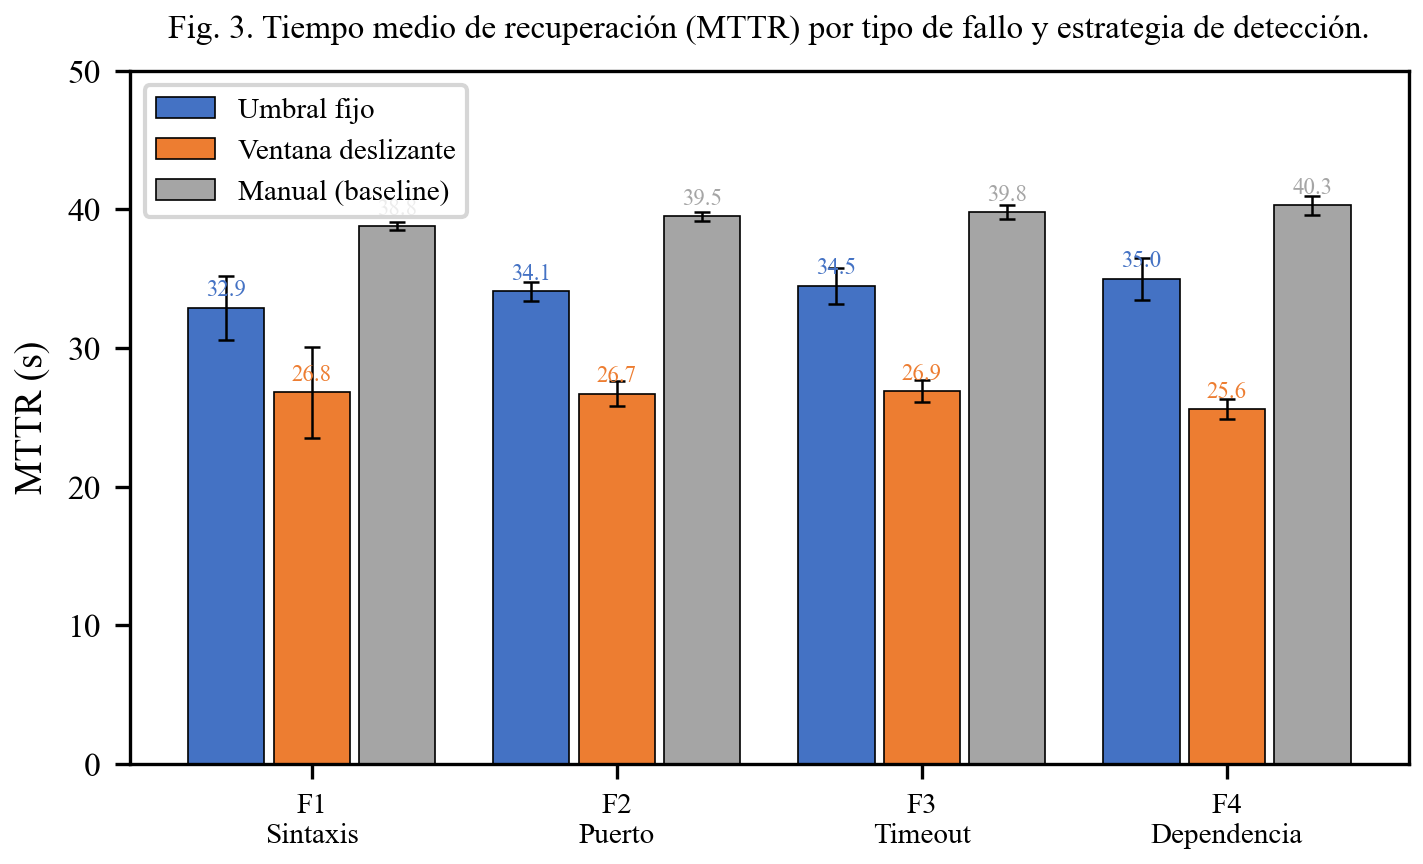
\includegraphics[width=\columnwidth]{images/fig3_mttr_barras.png}
\caption{Comparaci\'on del MTTR por tipo de fallo y estrategia de detecci\'on. Las barras representan el promedio y los segmentos indican una desviaci\'on est\'andar.}
\label{fig:mttr_barras}
\end{figure}

La Fig.~\ref{fig:boxplot} presenta la distribuci\'on completa de los tiempos de recuperaci\'on mediante diagramas de caja y bigotes, donde se observa la dispersi\'on de cada combinaci\'on. La estrategia de ventana deslizante no solo present\'o un MTTR promedio menor, sino tambi\'en una distribuci\'on m\'as compacta en los fallos de puerto cerrado, timeout y dependencia faltante, con rangos intercuart\'ilicos inferiores a 1.5~s. El fallo de sintaxis mostr\'o la mayor variabilidad en ambas estrategias autom\'aticas (desviaci\'on est\'andar de 3.3~s en ventana deslizante y 2.3~s en umbral fijo), atribuible a la naturaleza del fallo de construcci\'on que impide la creaci\'on del contenedor y depende de los tiempos de timeout del cliente HTTP.

\begin{figure}[t]
\centering
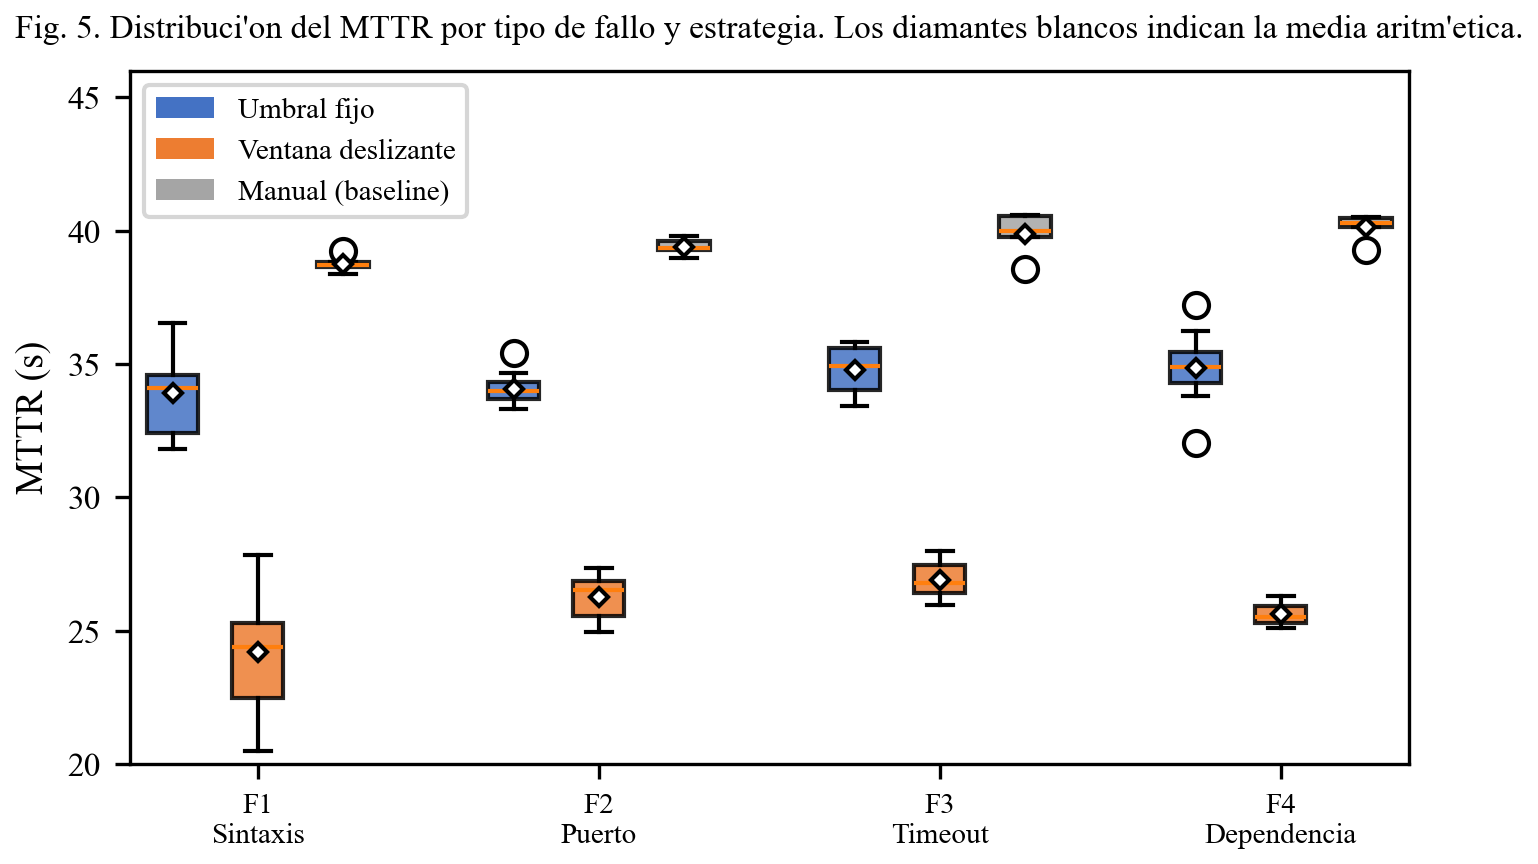
\includegraphics[width=\columnwidth]{images/fig5_boxplot.png}
\caption{Distribuci\'on del MTTR por tipo de fallo y estrategia. Los diamantes blancos indican la media aritm\'etica; las cajas abarcan el rango intercuart\'ilico.}
\label{fig:boxplot}
\end{figure}

En cuanto a la capacidad de detecci\'on, la Tabla~\ref{tab:deteccion} resume los resultados para cada estrategia. Las 40 corridas con fallo inyectado en cada estrategia autom\'atica fueron detectadas en su totalidad, y las 20 del baseline manual tambi\'en. No se registraron falsos negativos en ninguna combinaci\'on. Las corridas de control confirmaron que ninguna estrategia produce falsos positivos en ausencia de fallo.

\begin{table}[t]
\caption{Detecci\'on de Fallos y Falsos Positivos por Estrategia}
\label{tab:deteccion}
\centering\footnotesize
\resizebox{\columnwidth}{!}{%
\begin{tabular}{lcccc}
\hline
\textbf{Estrategia} & \textbf{Corridas} & \textbf{Detectados} & \textbf{Falsos negativos} & \textbf{Falsos positivos} \\
\hline
Umbral fijo       & 40 & 40/40 & 0 & 0/5 \\
Ventana deslizante & 40 & 40/40 & 0 & 0/5 \\
Manual (baseline) & 20 & 20/20 & 0 & -- \\
\hline
\end{tabular}
}
\end{table}

La reducci\'on del MTTR respecto a la intervenci\'on manual se calcul\'o tomando la estrategia autom\'atica de menor MTTR para cada tipo de fallo, que en todos los casos fue la ventana deslizante. La Tabla~\ref{tab:reduccion} presenta la comparaci\'on desglosada. La reducci\'on m\'inima fue de 30.9~\% (sintaxis) y la m\'axima de 36.5~\% (dependencia faltante), con un promedio de 33.0~\% entre los cuatro tipos de fallo.

\begin{table}[t]
\caption{Comparaci\'on de MTTR: Rollback Autom\'atico (Ventana Deslizante) versus Intervenci\'on Manual}
\label{tab:reduccion}
\centering\footnotesize
\resizebox{\columnwidth}{!}{%
\begin{tabular}{lccc}
\hline
\textbf{Tipo de fallo} & \textbf{MTTR autom\'atico (s)} & \textbf{MTTR manual (s)} & \textbf{Reducci\'on (\%)} \\
\hline
Sintaxis (build)      & 26.8 & 38.8 & 30.9 \\
Puerto cerrado        & 26.7 & 39.5 & 32.4 \\
Timeout health check  & 26.9 & 39.8 & 32.4 \\
Dependencia faltante  & 25.6 & 40.3 & 36.5 \\
\hline
\end{tabular}
}
\end{table}

\begin{figure}[t]
\centering
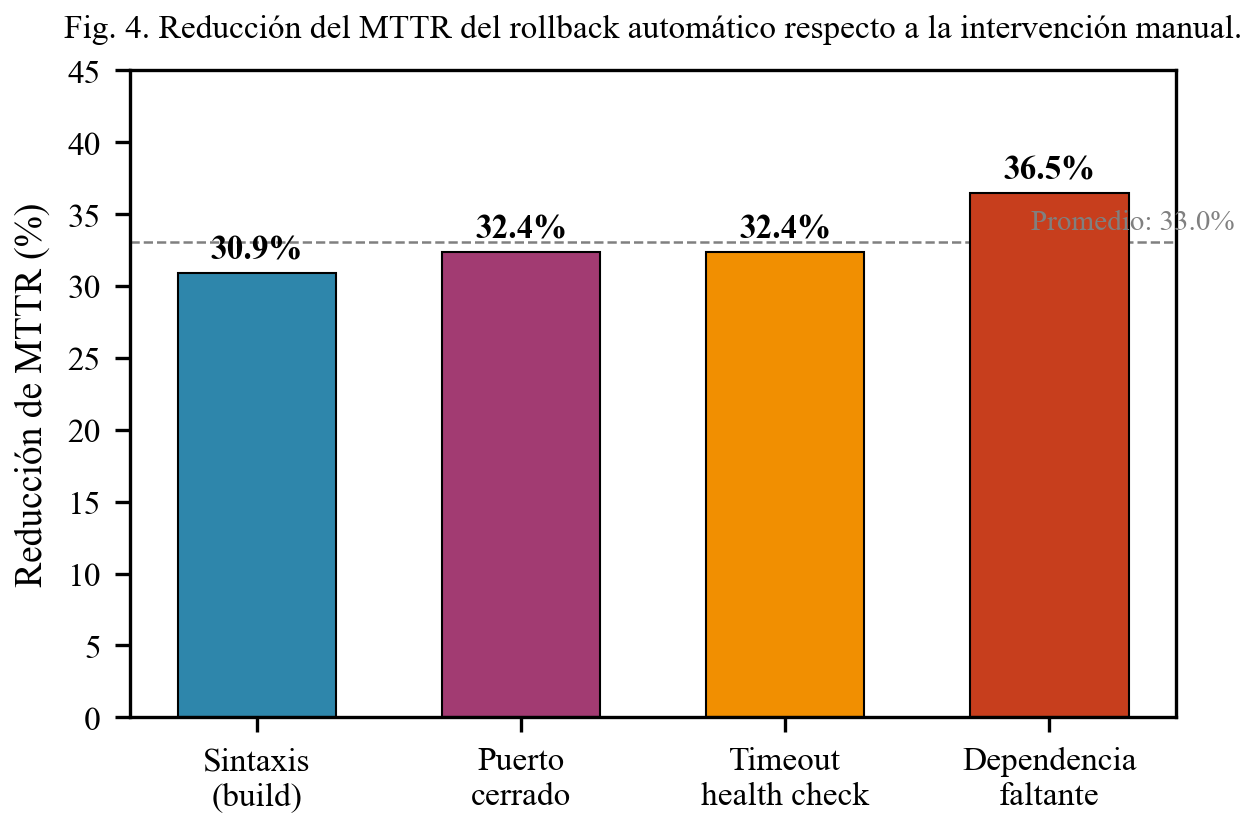
\includegraphics[width=\columnwidth]{images/fig4_reduccion.png}
\caption{Reducci\'on porcentual del MTTR del rollback autom\'atico respecto a la intervenci\'on manual, por tipo de fallo. La l\'inea discontinua indica el promedio global.}
\label{fig:reduccion}
\end{figure}

La Fig.~\ref{fig:cdf} presenta la funci\'on de distribuci\'on acumulada del MTTR para cada estrategia, agregando todos los tipos de fallo. La curva de la ventana deslizante se sit\'ua consistentemente a la izquierda de la del umbral fijo, lo que indica una mayor probabilidad de recuperaci\'on temprana en cualquier instante de tiempo. Por ejemplo, a los 30~s de monitoreo, la probabilidad de haber completado la recuperaci\'on es de aproximadamente 0.95 para la ventana deslizante, frente a 0.10 para el umbral fijo y 0.00 para la intervenci\'on manual.

\begin{figure}[t]
\centering
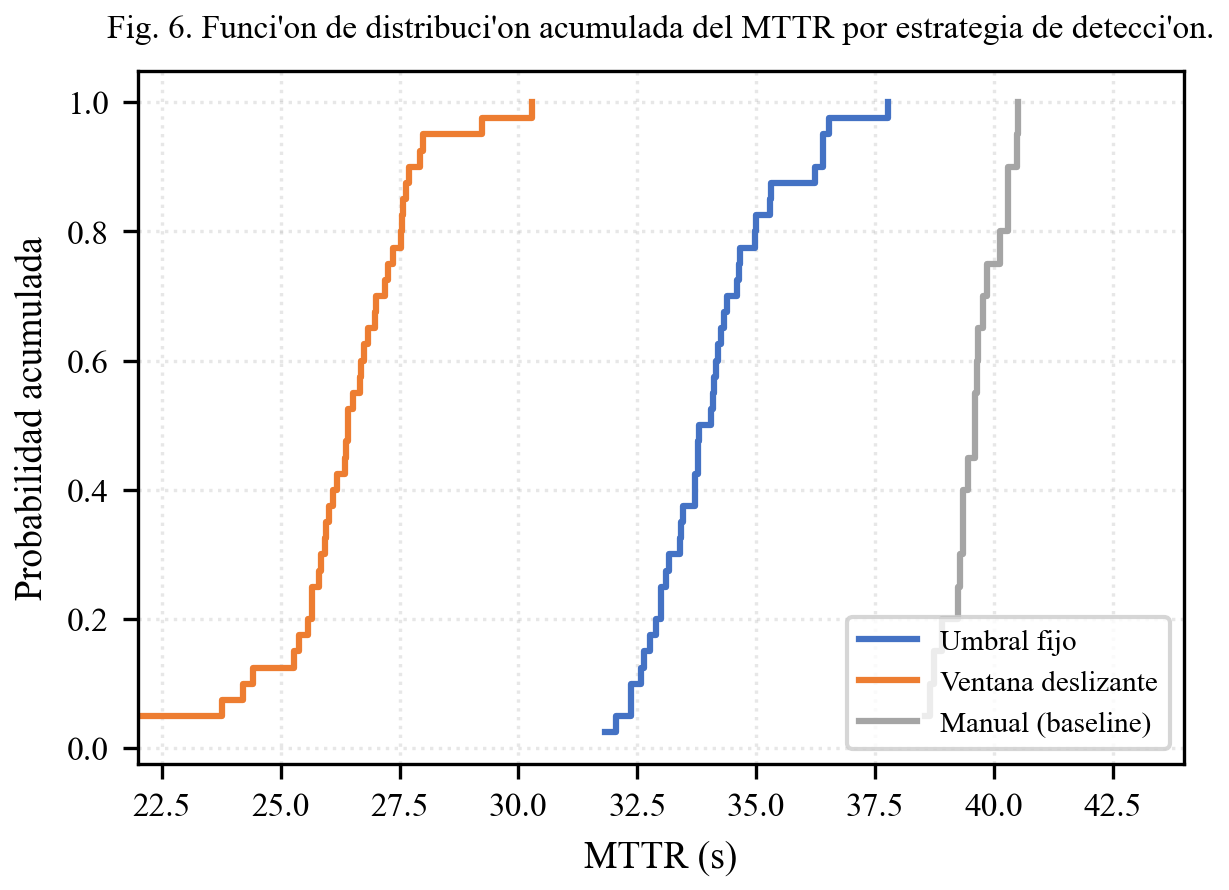
\includegraphics[width=\columnwidth]{images/fig6_cdf.png}
\caption{Funci\'on de distribuci\'on acumulada del MTTR por estrategia de detecci\'on. La curva de ventana deslizante domina estoc\'asticamente a las dem\'as.}
\label{fig:cdf}
\end{figure}

\subsection{Discusi\'on}

El resultado principal del experimento es que la estrategia de ventana deslizante produjo un MTTR menor que la de umbral fijo en los cuatro tipos de fallo evaluados, con una diferencia que oscil\'o entre 5.4~s y 9.4~s. Esta diferencia es atribuible a la capacidad de la ventana deslizante para tolerar fallos aislados sin activar la reversi\'on, reduciendo as\'i el tiempo perdido en ciclos de recuperaci\'on innecesarios. La ausencia de falsos positivos en las corridas de control sugiere que ninguna de las dos estrategias es propensa a activar reversiones en ausencia de fallo, al menos bajo las condiciones de prueba evaluadas.

La reducci\'on del MTTR respecto a la intervenci\'on manual alcanz\'o un promedio de 33.0~\% con la estrategia de ventana deslizante. Este valor es inferior al 50~\% reportado por Challa y Konatham~\cite{challa2024selfhealing} para su arquitectura de pipeline auto-reparable. La diferencia puede explicarse por el dise\~no del baseline manual en el presente estudio: en lugar de asumir un tiempo de diagn\'ostico y respuesta de un operador humano en un entorno de producci\'on real, se emple\'o una pausa fija calibrada en el mismo entorno de prueba, lo cual elimina la variabilidad propia de la intervenci\'on humana y reduce artificialmente la l\'inea base de comparaci\'on. Challa y Konatham no desglosan sus resultados por tipo de fallo ni comparan pol\'iticas de detecci\'on alternativas, por lo que no es posible determinar si la reducci\'on observada es uniforme entre categor\'ias de fallo o si depende del modo de fallo espec\'ifico.

Los resultados son consistentes con el an\'alisis de Hrusto et al.~\cite{hrusto2022optimization} sobre la importancia del contexto temporal en la decisi\'on de degradaci\'on. Si bien su estudio se centra en m\'etodos de aprendizaje profundo para la detecci\'on de anomal\'ias, el principio subyacente --una pol\'itica que incorpora informaci\'on temporal supera a una que opera exclusivamente sobre el instante presente-- se reproduce en el contraste entre umbral fijo y ventana deslizante. La magnitud de la diferencia observada (entre 18~\% y 27~\% de mejora relativa de la ventana deslizante sobre el umbral fijo, seg\'un el tipo de fallo) cuantifica la ventaja de incorporar memoria temporal en un contexto de pol\'itica simple, sin recurrir a modelos complejos de clasificaci\'on.

En cuanto a la taxonom\'ia de estrategias de reversi\'on propuesta por Avuthu~\cite{avuthu2021change}, el presente experimento aporta datos comparativos para dos de las modalidades que describe: la reversi\'on automatizada basada en umbrales de detecci\'on y la intervenci\'on manual. Los resultados confirman que la automatizaci\'on reduce el MTTR en todas las categor\'ias de fallo experimentadas. Sin embargo, la taxonom\'ia de Avuthu no distingue entre subestrategias de detecci\'on dentro de la reversi\'on automatizada; los resultados del presente estudio sugieren que esta distinci\'on es relevante, dado que la elecci\'on de la pol\'itica de detecci\'on (umbral fijo frente a ventana deslizante) introdujo diferencias de hasta 9.4~s en el MTTR.

Los resultados deben interpretarse a la luz de varias amenazas a la validez. En primer lugar, el experimento se ejecut\'o sobre un \'unico servicio en un entorno aislado, lo cual no refleja la complejidad de un sistema distribuido con m\'ultiples dependencias. En segundo lugar, los fallos inyectados son artificiales y fueron dise\~nados para ser detectables dentro del tiempo de espera configurado; los fallos reales de producci\'on pueden presentar perfiles m\'as sutiles o intermitentes. En tercer lugar, el tama\~no de muestra, aunque suficiente para el c\'alculo de estad\'isticos descriptivos, no permite realizar pruebas de significaci\'on estad\'istica robustas entre todas las combinaciones de condiciones. Finalmente, el intervalo de verificaci\'on de salud se fij\'o en 5~s para todas las condiciones; la variaci\'on de este par\'ametro podr\'ia alterar la relaci\'on entre las estrategias, favoreciendo potencialmente al umbral fijo en intervalos m\'as cortos o a la ventana deslizante en intervalos m\'as largos.

Pese a estas limitaciones, el estudio ofrece una contribuci\'on metodol\'ogica que complementa los trabajos citados: la construcci\'on de una matriz comparativa de tipos de fallo frente a estrategias de detecci\'on, con un grupo de referencia manual, repeticiones estad\'isticas y variables de control expl\'icitamente declaradas. Esta matriz puede servir como base para la selecci\'on informada de pol\'iticas de monitoreo en pipelines de despliegue, as\'i como para la replicaci\'on del experimento en entornos m\'as complejos.

\section{Conclusiones}

El experimento demostr\'o que la automatizaci\'on del mecanismo de reversi\'on reduce el tiempo medio de recuperaci\'on en todas las categor\'ias de fallo evaluadas, con una reducci\'on promedio del 33.0~\% respecto a la intervenci\'on manual. Asimismo, se observ\'o que la elecci\'on de la pol\'itica de detecci\'on influye en el MTTR: la ventana deslizante super\'o al umbral fijo en los cuatro tipos de fallo, con diferencias que oscilaron entre 5.4~s y 9.4~s.

La matriz comparativa construida a partir del dise\~no factorial permiti\'o desglosar el desempe\~no de cada estrategia por tipo de fallo, un nivel de detalle que no se encuentra en los estudios previos revisados. La inclusi\'on de un grupo de referencia manual y de corridas de control para la medici\'on de falsos positivos fortalece la validez interna del experimento, al permitir atribuir las diferencias observadas a la variable independiente y no a factores contextuales.

Las limitaciones del estudio --entorno simplificado, fallos artificiales y tama\~no de muestra acotado-- no invalidan los resultados obtenidos, pero definen el alcance de su generalizaci\'on.

El experimento completo, incluyendo los scripts de orquestaci\'on, la infraestructura como c\'odigo, el monitor de salud, los scripts de consolidaci\'on y las instrucciones de reproducci\'on, est\'a disponible en el repositorio del proyecto\footnote{\url{https://github.com/JECT-02/CI-CD-MONITOREO}} dentro del directorio \texttt{experimento/}. Cualquier investigador puede replicar el dise\~no factorial de 110 corridas ejecutando \texttt{runner.sh} en un entorno con Docker y Terraform, y consolidar los resultados con \texttt{consolidate.py}.

\section*{Reconocimientos}
% [PENDIENTE DE REDACCI\'ON -- Solo si corresponde]

\bibliographystyle{IEEEtran}
\bibliography{bibliografia/bibliografia}

\end{document}
